\documentclass[12pt]{article}%
\usepackage{amsmath,amssymb,amsthm,amsfonts}
\usepackage{wasysym}
\usepackage{graphicx}
\usepackage[dvipsnames]{xcolor}
\usepackage{stackengine}
\def\stackalignment{l}
\usepackage[colorlinks]{hyperref}
\usepackage{tikz}
\usepackage[export]{adjustbox}
\usepackage{graphicx}
\usepackage{indentfirst}
\usepackage{amsmath}
\usepackage{float}
\graphicspath{ {./} }

%\usepackage{geometry}
%\geometry{top = 0.9in}
\usepackage{appendix}

\newcounter{subfigure}

\newcommand{\R}{\mathbb{R}}
\newcommand{\C}{\mathbb{C}}
\newcommand{\N}{\mathbb{N}}
\renewcommand{\S}{\mathbb{S}^1}
\renewcommand{\Re}{\text{Re}}
\newcommand{\ea}{\textit{et al. }}
\renewcommand{\epsilon}{\varepsilon}
\renewcommand{\th}{\text{th}}
\newcommand{\sgn}{\operatorname{sgn}}

\renewcommand{\setminus}{\smallsetminus}

\newtheorem{thm}{Theorem}
\newtheorem{lemma}{Lemma}

\definecolor{red}{rgb}{0.8500, 0.3250, 0.0980}
\definecolor{green}{rgb}{0.4660, 0.6740, 0.1880}
\definecolor{yellow}{rgb}{0.9290, 0.6940, 0.1250}
\definecolor{blue}{rgb}{0, 0.4470, 0.7410}


\begin{document}

\title{Coding Project 1:  Detecting objects through frequency signatures}

\author{Jack Liu}
\date{}

\maketitle


\begin{abstract}
The Kraken lies beneath the ice in the Climate Pledge Area, and it is extremely difficult to detect directly due to other vibrations caused by the ice mountain and other objects under the ice. So, once we've collected the signal in the Climate Pledge Area, we'll need to use some ways to differentiate the Kraken from the other creatures lying under the ice. In this scenario, the Fourier transform and the Gussian filter are ideal approaches. They both help us to distinguish the Kraken signal from the other noise signals. In this report, we will go through the theoretical foundations of the Fourier transform and filtering. Python is also used to carry out the numerical solutions.
\end{abstract}


\section{Introduction}
\label{Sec: Intro}

Radar detection is a very useful tool in our daily lives. It was invented in the late 1930s. During World War II, radar played a critical role in the outcome of the war. It has also been employed in scientific studies to investigate the atmosphere, seas, and even the solar system. In addition, radar has been used in search and rescue operations, such as locating lost hikers or aircraft.

The radar detection is widely used in our daily life. For example,aviation, transportation, and meteorology. In here, we used it to detect Kraken at climate pledge area. Kraken is extremely difficult to detect directly due to other vibrations caused by the ice mountain and other objects under the ice. In this report, we will use the Radar detection technology with Fourier transform and the Gaussian filter to detect the Kraken from a lot of noise.

\section{Theoretical Background}
In this section, I will talk about what is the Fourier transform and the Gaussian filter with mathematical equations. I will also discuss techniques for dealing with spectral data.


\subsection{The Fourier Series}
Sine functions with harmonic dependence, sometimes referred to as components or harmonics, are added to form the Fourier series. A periodic function is the end result of the addition, and its functional form is defined by the sum of the parameters for its amplitude and phase, as well as the length (or period) of the period, the number of components, and the number of components.
So it is a way to represent a periodic function as a sum of sine and cosine, and the general form is:
\begin{equation}
    f(x) = \frac{a_0}{2} + \sum_{n=1}^{\infty} [a_n \cos(\frac{n\pi x}{L}) + b_n \sin(\frac{n\pi x}{L})]
\end{equation}

\noindent where $a_0$, $a_n$ and $b_n$ are constants determined by the function $f(x)$.

Multiplying the function $f(x)$ by $\cos(mx)$ on both side and integrating over the interval $[-L, L]$ gives:
\begin{equation}
    \int_{-L}^{L} f(x) \frac{\cos(m\pi x)}{L} dx = 2L  \qquad
    if \; m = 0 
\end{equation}

\begin{equation}
\int_{-L}^{L} f(x) \frac{\cos(n\pi x)}{L} \frac{\cos(m\pi x)}{L} =
    \begin{cases} 
        L & n = m \\
        0 & n \le m \
    \end{cases}
\end{equation}

The coefficients $a_n$ and $b_n$ can be found using the following formulas:
\begin{equation}
    a_n = \frac{1}{L} \int_{-L}^{L} f(x) \cos(\frac{n\pi x}{L}) dx
\end{equation}

\begin{equation}
    b_n = \frac{1}{L} \int_{-L}^{L} f(x) \sin(\frac{n\pi x}{L}) dx
\end{equation}
An complex version will also help us do some calculations. From Euler's formula:
$$e^{i \omega t} = \cos(\omega t) + i \sin(\omega t)$$
we can write the series in a new form:
\begin{equation}
    f(x) = \sum_{n=1}^{\infty} c_n e^{i\frac{n\pi x}{L}} \qquad x \in [-L, L]
\end{equation}
and by doing some algebra, we can get the coefficients $c_n$:
\begin{equation}
    c_n = \frac{1}{2L} \int_{-L}^{L} f(x) e^{-i\frac{n\pi x}{L}} dx
\end{equation}
Now the Fourier series is complex but the function $f(x)$ still to be real.


\subsection{The Fourier Transform}
The Fourier transform is a mathematical technique that can be used to transform a function from the time domain to the frequency domain. It is an integral transform define over $x \in [-\infty, \infty]$. 

With Euler's method we talked above, We can represent a signal in the frequency domain. Specifically, we can decompose a signal $f(t)$ into a sum of complex exponentials, each with a different angular frequency:
$f(x) = \sum_{k = -\infty}^{\infty} c_k e^{i k x}$

Basically, we took our Fourier series and make it infinite form. We can write it as:
\begin{equation}
    F(k) = \int_{-\infty}^{\infty} f(x)e^{-i k x} dx
\end{equation}
And this is the Fourier Transform and our coefficient become our function and summation become integral. 

The inverse Fourier Transform is:
$f(x)=\int_{-\infty}^{\infty} F(k) e^{i k x} dk$



\subsection{The Fast Fourier Transform}

Fast Fourier Transform is an algorithm that is used to efficiently compute the discrete Fourier transform. DFT used to be very slow, it take order of $N^2$ time to compute. But FFT can do it in order of $NlogN$ time. So FFT is way more efficient. In this project, we use FFT to compute the Fourier transform in Python. The library that and carry out FFT is numpy.fft.fft() in 2D space and numpy.fft.fftn() in higher dimension. 

\subsection{Spectral Averaging}

In the first part of the project, we use spectral averaging to remove the noise in the data. Since we have multiple signal in the data and a lot of noise in each signal, we can use spectral averaging to lower the noise level. Because noise is random(some where could be 0.9 but other palce could be 0), so when we average the data, the noises are going to dampen. Since regular signal always have the same amplitude, so the signal will not be affected by the averaging.


\subsection{Spectral Filtering}

Spectral filtering is a technique used in signal processing. It allow us to extract specific frequency components from a signal. It can be done by apply the filter to the signal in the frequency domain. Usually, we first use Fourier Transform to convert the signal from the time domain to the frequency domain, apply the filter and then converting the filtered signal back to the time domain using an inverse Fourier transform.

In order to detect Kraken we use Gaussian filter which defined as:
\begin{equation}
    F(k) = e^{-\tau(k - k_0)^2}
\end{equation}
This function is a Gaussian function in the frequency domain, where $k$ is the frequency variable, $k_0$ is the center frequency, and $\tau$ the bandwidth of the filter. 

In this project, this filter is a type of low-pass filter and it eliminates high-frequency components. We use 1/L as the bandwidth and max frequency after averaging the signal as the center frequency. This filter is used to remove the high-frequency noise in the data.

\section{Numerical Methods}

In the first part of the code, we create a 3D location box that represent Climate Pledge Area. Also we create frequency array with rescale them to be 2pi periodic and shift values to order them correctly. (line 10-29)

Then we start to averaging the signal to clean the noise. Since Kraken data is not 3D version, and it contains 262144 rows and 49 columns, each column have the signal in x, y, z direction, so we need to reshape the data to (64, 64, 64)(x-y-z) 49 times. Then we use FFT in each columns and sum up together then divide by 49 to get the average. After averageing, we can find where is the peak frequency and using that as our center frequency for Gussian filter.(line 36-51)

Since we have 3 direction, we need to find filter for each direction(line 55-63) then combine them together. Also since Gussian is exponential, so adding is same as multiplying. (line 66-73)

After we get the filter, we can apply it to the data. We use FFT to convert the data to frequency domain, then multiply the filter with the data and convert it back to time domain. Then find the peak in the time domain which will give us the location of Kraken (line 67-78)

The rest of the code are just make visulaization for the data we filtered in line 67-78. We use 3D plot to show the location of Kraken and 2D plot to show the location of Kraken in x-y plane.

\section{Results}
In this section, I'll include two graphs and one table that depict the Kraken's route that we discussed before. Figure 1 displays the Kraken's 3D position. Kraken's depth beneath the ice is shown on the z axis. Each dot depicts Kraken's location at a certain time. We can see that Kraken move in a helical shape and break through the ice. Each point in the graph is a good position to land a check.
\begin{figure}[H]
    \centering
    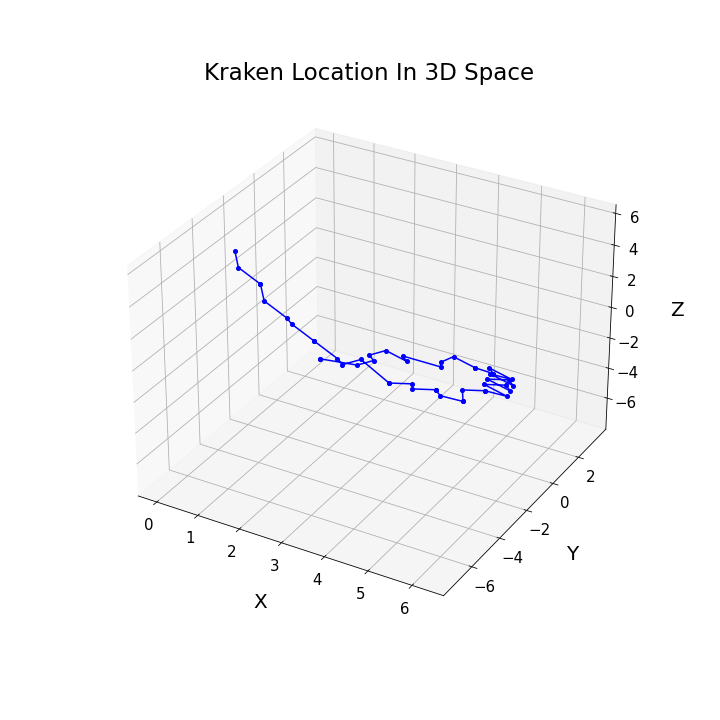
\includegraphics[width=1\textwidth]{Kraken location.png}
    \caption{Kraken location}\label{fig:kraken_location}
\end{figure}

Figure 2 is the same as Figure 1, except it is projected to the x-y plane. This graph makes it clearer for us where to land the check. Each point in the x-y plane may be thought of as having a location on the ground. Since we want to pinpoint the Kraken's movement in ground to do a hard check on it, the z direction information is not present in the projection since it is not crucial in this circumstance. 
\begin{figure}[H]
\centering
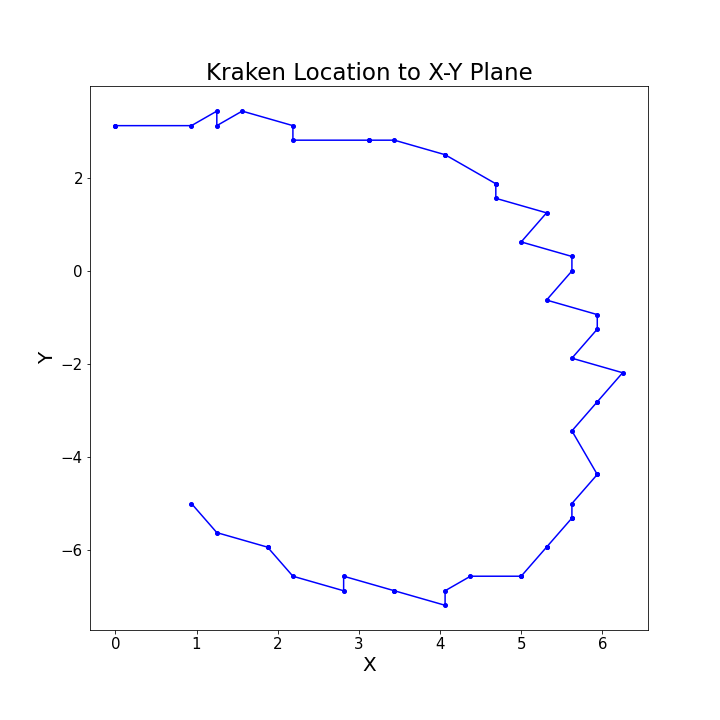
\includegraphics[width=1\textwidth]{projection.png}
\caption{Projection to x-y plane}\label{fig:projection}
\end{figure}

The numerical value for each point is displayed in Table 1. The Kraken's location's x and y coordinates make up the first two components, while its depth makes up the third. Based on this table, we construct the plot. It provides just as a guide for us to look up the Kraken's precise position.
\begin{table}[H]
    \centering
    % To place a caption above a table
    \caption{Numerical Data of Kraken's Location}
    \begin{tabular}{|l|l|l|}
        \hline
            X & Y & Z \\ \hline
            0.0 & 3.125 & -7.8125 \\ \hline
            0.0 & 3.125 & -7.8125 \\ \hline
            0.9375 & 3.125 & -7.5 \\ \hline
            1.25 & 3.4375 & -7.1875 \\ \hline
            1.25 & 3.125 & -6.5625 \\ \hline
            1.5625 & 3.4375 & -6.25 \\ \hline
            2.1875 & 3.125 & -6.25 \\ \hline
            2.1875 & 2.8125 & -5.625 \\ \hline
            3.125 & 2.8125 & -5.625 \\ \hline
            3.125 & 2.8125 & -5.3125 \\ \hline
            3.4375 & 2.8125 & -4.6875 \\ \hline
            4.0625 & 2.5 & -4.6875 \\ \hline
            4.0625 & 2.5 & -4.6875 \\ \hline
            4.6875 & 1.875 & -4.0625 \\ \hline
            4.6875 & 1.875 & -4.0625 \\ \hline
            4.6875 & 1.5625 & -3.4375 \\ \hline
            5.3125 & 1.25 & -3.4375 \\ \hline
            5.0 & 0.625 & -2.8125 \\ \hline
            5.625 & 0.3125 & -2.8125 \\ \hline
            5.625 & 0.0 & -2.1875 \\ \hline
            5.3125 & -0.625 & -1.875 \\ \hline
            5.9375 & -0.9375 & -1.875 \\ \hline
            5.9375 & -1.25 & -1.25 \\ \hline
            5.625 & -1.875 & -0.9375 \\ \hline
            6.25 & -2.1875 & -0.9375 \\ \hline
        \end{tabular}
        \begin{tabular}{|l|l|l|}
            \hline
            X & Y & Z \\ \hline
            5.9375 & -2.8125 & -0.3125 \\ \hline
            5.9375 & -2.8125 & -0.3125 \\ \hline
            5.625 & -3.4375 & 0.0 \\ \hline
            5.9375 & -4.375 & 0.3125 \\ \hline
            5.9375 & -4.375 & 0.3125 \\ \hline
            5.625 & -5.0 & 0.9375 \\ \hline
            5.625 & -5.3125 & 1.5625 \\ \hline
            5.625 & -5.3125 & 1.5625 \\ \hline
            5.3125 & -5.9375 & 1.875 \\ \hline
            5.3125 & -5.9375 & 2.1875 \\ \hline
            5.0 & -6.5625 & 2.5 \\ \hline
            5.0 & -6.5625 & 2.5 \\ \hline
            4.375 & -6.5625 & 3.4375 \\ \hline
            4.0625 & -6.875 & 3.125 \\ \hline
            4.0625 & -7.1875 & 3.75 \\ \hline
            3.4375 & -6.875 & 4.0625 \\ \hline
            3.4375 & -6.875 & 4.0625 \\ \hline
            2.8125 & -6.5625 & 4.375 \\ \hline
            2.8125 & -6.875 & 5.0 \\ \hline
            2.1875 & -6.5625 & 5.3125 \\ \hline
            1.875 & -5.9375 & 5.625 \\ \hline
            1.875 & -5.9375 & 5.625 \\ \hline
            1.25 & -5.625 & 5.9375 \\ \hline
            0.9375 & -5.0 & 6.25 \\ \hline
        \end{tabular}
\end{table}



\section{Conclusion}\label{Sec: Conclusion}

We can distinguish Kraken from the other noise-making things lying beneath the ice by applying the Fourier Transform and the Gussian filter. The method we utilize here is quite similar to radar detection. The Gussian filter is used to remove noise while retaining the Kraken signal. And by using Fourier Transform, we are able to transform the signal to frequency domain. Then, after applying the filter, we can seek for the actual Kraken signal by looking at the peak frequency. Finally, we can determine the Kraken's path and the ideal spot on the ice would be optimal for a defenceman to be to make a hard check on the Kraken.

After doing this project, I learned how to use Fourier Transform in a real situation not just calculating the numbers. I also learned how to use the Gussian filter to remove noise. Also, I learned a lot of librarys in python that can carry out numerical solutions and plot in 3D.


\section*{Acknowledgment}

Thanks Katie for answaring the general question and Michael for helping me with the python.


\end{document}
